
\section{Comparison with the Hypothesis Corpus}
\label{sec:dataset-hc}

\begin{table}[t]
\centering
\begin{minipage}[t]{0.36\textwidth}
  \centering
  \caption{PBT corpus statistics.}
  \label{tab:dataset-stats}
  \footnotesize
  \begin{tabular}{lr}
    \toprule
    \textbf{Metric} & \textbf{Value} \\
    \midrule
    PBTs (raw scrape)              & 54{,}345 \\
    PBTs (post-dedup)              & 11{,}039 \\
    Unique repositories            & 333 \\
    Unique GitHub owners           & 281 \\
    Upstream project names         & 303 \\
    Top-1 / top-10 PBT share       & 8.7\% / 58.5\% \\
    \midrule
    \multicolumn{2}{@{}l}{\emph{Per-repo (min / med / max):}} \\
    PBTs per repo                  & 1 / 6 / 956 \\
    Stars                          & 0 / 0 / 9{,}438 \\
    Forks                          & 0 / 0 / 1{,}567 \\
    \midrule
    \multicolumn{2}{@{}l}{\emph{Per-PBT (min / med / max):}} \\
    PBT LoC                        & 2 / 13 / 174 \\
    Direct fn deps                 & 0 / 1 / 15 \\
    \bottomrule
  \end{tabular}
\end{minipage}\hfill
\begin{minipage}[t]{0.62\textwidth}
  \centering
  \setlength{\tabcolsep}{3pt}
  \caption{Comparison with HC-2026~\cite{devoe2026hypothesis}.}
  \label{tab:dataset-comparison}
  \footnotesize
  \begin{tabular}{@{}l c c@{}}
    \toprule
    & \textbf{\FVSpec:PBT} & \textbf{HC-2026} \\
    \midrule
    Discovery        & dep.\ graph        & GitHub search \\
    Raw PBTs         & 54{,}345           & 38{,}885 \\
    Tests (deduped)  & 11{,}039           & 23{,}139 \\
    Repos            & 333                & 1{,}504 \\
    Repo dedup       & fork/name          & \texttt{is\_fork} \\
    Test dedup       & SHA-256            & parametrization \\
    License filter   & no copyleft        & none \\
    Per-test data    & source + metrics   & runtime + coverage \\
    \midrule
    Repo overlap (valid)  & \multicolumn{2}{c}{28 / 333 \enskip(8\%)} \\
    Repo overlap (any)    & \multicolumn{2}{c}{111 / 333 \enskip(33\%)} \\
    \bottomrule
  \end{tabular}
\end{minipage}
\end{table}

While we were finalizing this work, the Hypothesis maintainers released their own scraped corpus~\cite{devoe2026hypothesis} (HC-2026).
The two corpora target different downstream uses---HC-2026 is built to study Hypothesis \emph{runtime} behavior (entropy consumption, predicate firing, coverage), while ours is built to feed a Lean formalization pipeline---which drives the design differences summarized in Table~\ref{tab:dataset-comparison}.
A consequence of HC-2026's runtime focus is that it filters out as ``invalid'' any repository whose PBTs may not be directly runnable without some custom setup: code that depends on external services, API keys, environment variables, or live databases. Our pipeline imposes no such requirement, since we only need a PBT's source code to translate it into Lean. Of our 333 repositories, 28 appear in HC-2026's valid (executable) set and 111 (33\%) appear in the pre-validity superset---meaning roughly 80 of our repositories were dropped by HC-2026 for being too operationally entangled to run, consistent with our goal of producing challenging and realistic FV problems.
Future work could merge the two corpora to enlarge the input pool; we did not pursue this here because the present token budget does not exhaust even our own 11{,}039-PBT corpus.

\section{Axiomatization Details}
\subsection{Axiomatized Interfaces for Effectful Code}
\label{sec:threats-axioms}

The \texttt{isort} running example from \Secr{task} is deliberately pure. Most PBTs in our corpus are not: production code routinely touches Redis, sockets, the filesystem, the wall clock, webhook queues, and so forth. A natural objection is that any Lean theorem extracted from such a PBT cannot say anything meaningful about the live system.

The formalization agent handles this by treating the effectful world as an \emph{uninterpreted interface}. Parts of the source essential to the property---the entities and operators it constrains---are translated into Lean structures and inductive types. Parts that are pure plumbing---the database, the queue, the system clock---are introduced as opaque \texttt{axiom} declarations and threaded through the theorem as parameters. The resulting theorem holds \emph{over all interpretations} of those axioms, which is exactly the contract the original PBT was checking against the live environment.

A canonical instance is \texttt{test\_workflow\_job\_time\_to\_start} from \texttt{scality/runner-manager}\footnote{\url{https://github.com/scality/runner-manager}}, a GitHub Actions self-hosted runner controller. The Python PBT initializes Redis-backed model classes, runs an ORM migrator, calls \texttt{datetime.now()} to fabricate two timestamps straddling a runner-startup timeout, enqueues a webhook through a background job queue, and asserts on the resulting runner count. The \FVSpec translation introduces seventeen axioms---including \texttt{Redis}, \texttt{Queue}, \texttt{State}, \texttt{State.after\_enqueue}, and \texttt{get\_runners}---and states the contract purely in terms of these uninterpreted operators:

\begin{lstlisting}[style=code, language=Lean, basicstyle=\ttfamily\scriptsize]
theorem create_runner_when_above_timeout
  (initial_state : State) (state_after_enqueue : State)
  (runner_group : RunnerGroup) (webhook_updated : WorkflowJobEvent)
  (settings : ExtendedSettings) (created_at started_at : Time)
  (h_initial_count : (get_runners runner_group initial_state).length = 1)
  (h_below_max     : 1 < runner_group.max)
  (h_above_timeout : started_at - created_at > settings.timeout_runner)
  (h_enqueue       : state_after_enqueue =
    State.after_enqueue initial_state runner_group webhook_updated settings)
  : (get_runners runner_group state_after_enqueue).length = 2 := sorry
\end{lstlisting}

A model proving \texttt{create\_runner\_when\_above\_timeout} is reasoning about a scheduler's state-transition semantics under a timeout precondition; the fact that the production scheduler talks to Redis is no more load-bearing in the theorem than the choice of register allocator is in a correctness proof of a sorting algorithm.

\subsection{Where Axiomatization Breaks Down}
\label{sec:threats-axiom-limits}

The axiomatization move is not a universal solvent.

\emph{Properties about the effect itself.} If the property is fundamentally about timing, memory, ordering of side effects, or wall-clock latency, an uninterpreted axiom cannot witness it. \texttt{assert response\_time < 100ms} cannot become a meaningful Lean theorem because the relevant semantics is precisely what the axiomatization discards.

\emph{Effectful code disguised as pure code.} The agent identifies effectful boundaries via type signatures and call patterns. When a function has a pure signature but performs side effects internally (e.g., a logger called via a global, an \texttt{lru\_cache}-style hidden state), the agent will inline it as if pure. The resulting theorem may compile and even be true, but its proof obligation does not constrain the original side-effecting behavior.

\emph{Axioms that misrepresent the API contract.} \texttt{axiom Redis : Type} captures \emph{some} Redis but not the real one. The agent does not encode Redis's consistency guarantees, ordering, or failure modes. A theorem proven over the axiomatized interface may not transfer to the live system if the production code relies on those omitted guarantees.

\section{\FVSpec:FV Grader Distributions}

\ref{fig:difficulty_distribution} shows difficulty distribution according to the Haiku 4.5 grader. \ref{fig:difficulty_vs_faithfulness} shows difficulty grade against output characteristics and LoC. 

\begin{figure}[t]
  \centering
  
\includegraphics[width=\linewidth]{figs/difficulty_distribution.pdf}
  \caption{Difficulty distribution: easy vs.\ hard counts (left) and grader confidence distribution (right). $n$ shown in title.}
  \label{fig:difficulty_distribution}
\end{figure}

\begin{figure}[t]
  \centering
  
\includegraphics[width=\linewidth]{figs/difficulty_vs_faithfulness.pdf}
  \caption{Difficulty vs.\ output characteristics: overall faithfulness (left) and total Lean lines (right), stratified by difficulty.}
  \label{fig:difficulty_vs_faithfulness}
\end{figure}

\section{\FVSpec:FV Number of Theorems and Complexity per Sample} \label{appndx:complexity}

\ref{fig:lean_complexity} shows the median sample contains multiple theorems each requiring an independent proof, and the \texttt{sorry} count tracks the theorem count closely, as expected from our pipeline design.

\begin{figure}[t]
  \centering
  
\includegraphics[width=\linewidth]{figs/lean_complexity.pdf}
  \caption{Lean output complexity: total lines (left), theorems per sample (center), and \texttt{sorry} placeholders per sample (right). Tail counts and maxima shown in axis labels.}
  \label{fig:lean_complexity}
\end{figure}

\section{\FVSpec:PBT Code Quality Metrics}

Figure~\ref{fig:python_source} summarizes three code-quality metrics across the corpus.
The source tests span a wide range of complexity, from trivial single-assertion tests to multi-strategy tests exercising complex library APIs---diversity inherited directly from real-world engineering practice and not curated for difficulty.

\begin{figure}[t]
  \centering
  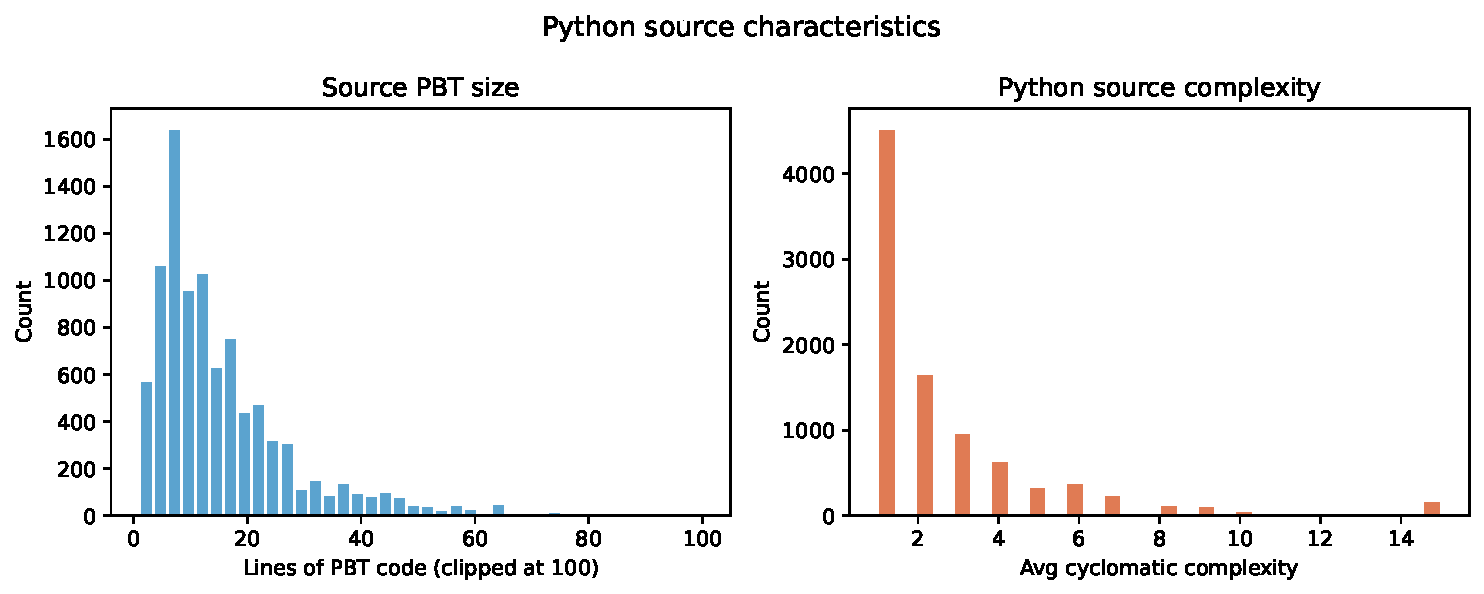
\includegraphics[width=\linewidth]{figs/python_source.pdf}
  \caption{Code-quality metrics for the 11{,}039 deduplicated PBTs, computed by Radon~\cite{radon}. \emph{Left}: lines of code.
  \emph{Center}: cyclomatic complexity---the number of linearly independent execution paths through the function, i.e.\ one plus the number of binary branch points~\cite{mccabe1976complexity}; higher values indicate more complex control flow.
  \emph{Right}: maintainability index---a 0--100 composite of Halstead volume~\cite{halstead1977elements}, cyclomatic complexity, and source lines, where higher is more maintainable; the spike at 100 is an artefact of Radon capping the score at that value.}
  \label{fig:python_source}
\end{figure}

\section{\FVSpec:FV Pipeline Cost} \label{appndx:pipeline_cost}

Per-sample pipeline cost is right-skewed (Figure~\ref{fig:pipeline_cost}): most samples compile within a few agent turns, but a tail of difficult translations requires many repair iterations before the Lean LSP reports success or the budget is exhausted.

\begin{figure}[t]
  \centering
  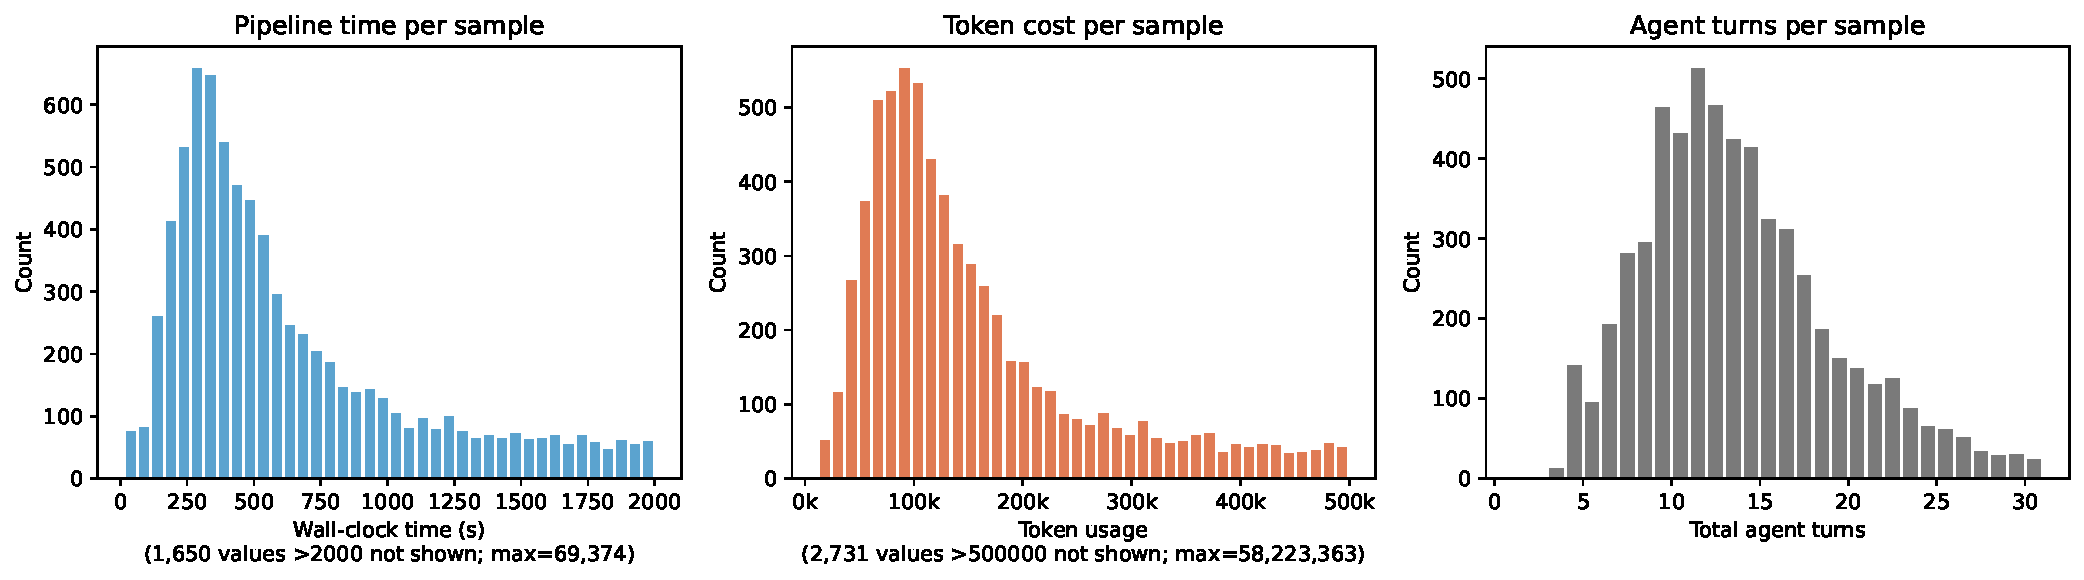
\includegraphics[width=\linewidth]{figs/pipeline_cost.pdf}
  \caption{Pipeline cost per sample: wall-clock time (left), token usage (center), and agent turns (right). Tail counts and maxima shown in axis labels.}
  \label{fig:pipeline_cost}
\end{figure}